\documentclass{cssspaper}
% \卒論
\修論
% \usepackage{epsbox}
\usepackage{makeidx}
\usepackage{verbatim}
\usepackage{enumitem}
\usepackage[dvipdfmx]{graphicx}
\usepackage{listings,jvlisting}
  \title {C言語ソースコードのコードフロー可視化による\\制御構造理解支援システムの構築}
   \author{小方 亮人}
   \teacher{香川 考司}
   \chief{香川 考司}
	 \seconda{安藤 一秋}
	 \secondb{高木 智彦}
   \year{令和6年度~(2024年度)}
\date{令和7年1月30日}
% \date{\today}

\lstset{
    basicstyle={\ttfamily},
    identifierstyle={\small},
    commentstyle={\smallitshape},
    keywordstyle={\small\bfseries},
    ndkeywordstyle={\small},
    stringstyle={\small\ttfamily},
    frame=single,
    % framexleftmargin=1em,
    breaklines=true,
    columns=[l]{fullflexible},
   %  numbers=left,
    xrightmargin=3zw,
    xleftmargin=3zw,
    % xleftmargin=3zw,
    numberstyle={\scriptsize},
    % framesep=5pt,
    stepnumber=1,
    numbersep=1zw,
    lineskip=-0.5ex
}

% \makeindex

\begin{etitleenv}
  Implementation of a Support System for Understanding Control Structures
  through Code Flow Visualization of C Language Source Code.
\end{etitleenv}

\begin{eabstract}
Novice programmers often struggle to understand error messages and 
spend considerable time identifying what is wrong with their code.
To address this issue and help beginners efficiently learn and 
acquire appropriate programming skills, effective educational support is necessary.
In particular, a system that identifies error locations, 
provides immediate feedback, and suggests improvement methods is considered 
to be highly beneficial.
One of the challenges in programming education is that novice learners often 
have an insufficient understanding of the "flow of control" in code.
To solve this problem, this study develops a web-based feedback system.
The system analyzes the input source code, identifies errors, 
and provides line numbers and guidance on how to fix them.
Additionally, it visually displays the flow of control, 
allowing beginners to intuitively understand how the code flows.
The system uses The language-c-quote library of Haskell for source code analysis, 
offering the advantage of easy extensibility for further analysis tasks. 
Through this system, the study aims to support novice learners and promote 
efficient and effective programming education.

\end{eabstract}

\begin{jabstract}

プログラミングを始めたばかりの学習者は、エラー内容の理解が難しく、
何が間違っているのかを見つけるのに多くの時間を費やすことがよくある。
このような課題に対処し、初学者が効率的に学びながら適切なプログラミング技術を
身につけるためには学習をサポートする効果的な教育支援が必要である。
特に、エラー箇所を特定して即座にフィードバックを提供し、
改善方法を提示する仕組みが有効と考えられる。
またプログラミング教育における課題の一つとして、初学者が「コードの流れ」を
十分に理解できていない点が挙げられる。本研究ではこの課題を解決するために、
Webベースのフィードバック提供システムを開発した。このシステムは、
入力されたソースコードを構文解析し、エラー箇所を特定して行番号や修正の指針を提示する。
また、制御フローの流れを視覚的に表示することで、
初学者がコードの流れを直感的に理解できるように設計されている。
ソースコード解析にはHaskellのlanguage-c-quoteを用いており、
解析項目の拡張が容易である点も特徴である。このシステムを通じて、
初学者の学習を支援し効率的で効果的なプログラミング教育を目指す。

\end{jabstract}

\begin{keyword}
  Haskell,構文解析,制御構造,プログラミング学習支援,ソースコード解析
\end{keyword}

\begin{document}
\maketitle
%  \listoffigures % 図の目次
%  \listoftables  % 表の目次

    \chapter{はじめに}
        \section{プログラミング初学者の課題}
        大学で情報系の専門課程に進むと、ほとんどの学生がプログラミングの基礎を
        学ぶことになるが、高校で「情報I」が必修化された現在でも、
        プログラミングの経験が浅い学生や本格的なプログラミングを
        初めて学ぶ学生が多いのが現状となっている。
        初学者がプログラムに関する基礎的なスキルを短期間で習得することは容易ではなく、
        多くの学生が学習を進める中で自身が記述したコードに関するエラーや警告に対して
        悪戦苦闘することになる。そこで発生したエラーの解決は初学者にとって、
        単なる間違いを直す作業ではなく、問題の本質を理解しその原因を突き止めることが
        重要である。しかしプログラミングを始めたばかりの学習者はエラーの内容が理解できず、
        何が間違っているのかを特定するのに多くの時間を費やしてしまうことが多々ある。
        その結果学習が遅れ、モチベーションの低下を招くことにもつながってしまう。
        中にはコンパイルエラーとして表示されないミスもあり、これらを初学者が自力で
        正確に把握し修正することはとても難しい問題となっている。
        これらのエラーの多くは初学者が陥りやすい些細なミスに起因していることが
        多いため、その修正方法をひとつひとつ丁寧に指導することは学習者にとっても
        教育者にとっても大きな負担となる。このような学習過程において教育者が
        全ての学習者に個別にフィードバックを提供することは難しく、大人数のクラスや
        自己学習環境では特に困難となっている。学習者が自分で改善方法を見つけられない
        状況が続くと、プログラミングに対する苦手意識が強まり、その後の学習にも
        悪影響を及ぼすことになる。
        
        \section{プログラミング学習支援ツールの必要性}
        前述の課題より、プログラミング教育においては、
        学習者が効率的に学び適切なプログラミング技術を身につけるための教育支援が
        必要である。特に、間違っている箇所を特定し即座にフィードバックを与え、
        改善方法を迅速に提供することのできるものが効果的であると考えられる。
        このようなフィードバックは学習者が自らコードを改善するための指針を提供し、
        自己修正能力を高めるだけではなく、プログラミング学習に対する自信をも
        促進することが期待される。
        しかし現状ではそのようなコード指摘ツールにはいくつかの課題が存在する。
        多くのツールは専門家向けに設計されており、その出力は初学者にとって
        直感的ではなく理解しづらいものが多いため、そのまま学習者が活用することは
        困難である。また、初学者がよく犯すミスに対して柔軟に対応できるツールの開発が
        求められているが、既存のツールではそのような対応が十分ではなく、
        初学者に適切なフィードバックを提供するための機能が不足している。
        このような背景の中で、初学者に特化したプログラミング学習支援ツールの開発は、
        プログラミング学習の理解を深め、効率的な学習を促進させるために重要な課題である。

        \section{コードの流れに対する理解不足がもたらす影響}
        またプログラミング教育における初学者の学習過程では、特に「コードの流れ」に
        対する理解が未熟であることが課題の一つとなっている。
        プログラムの制御の流れを理解することがプログラミング教育において重要な課題であり、
        初学者はしばしば制御構文の理解に苦しむ。
        プログラムは単に記述された命令が順番に実行されるわけではなく、
        制御構文によってその流れが動的に変化するものであるが、
        初学者の中にはこの制御構文を正しく理解できず、何故そのような
        流れになるのかが判断できていなかったり、意図的に利用することが
        難しいと感じてしまったりしている人が多い。
        制御構文の理解不足は、コードがどのように動作しているのかが
        理解できなくなる原因となり、その結果としてプログラムの結果が
        予期しないものとなることで効率的なデバッグも行えず、
        プログラミング学習の進行が遅れることに繋がる。
        したがって、制御構文やコードの流れを直感的に理解できるような支援が重要である。

        % そこで、学習者のコードへの指摘を行う支援ツールの開発に取り組んだ研究として、
        % C-Helper \cite{1,2,3}や、それを用いた島川の研究 \cite{4}が挙げられる。
        % しかしC-HelperではJavaを実装言語として採用し、構文解析の結果として
        % 得られる抽象構文木を操作するために、Visitorパターンというデザインパターンを
        % 利用している。この方法では抽象構文木に新しいデータ構造や機能を追加する際に、
        % 新しいメソッドの追加や各クラスにそのメソッドに応じた実装を追加する必要がある。
        % この制約により、C-Helperのアプローチは調査項目の拡張性において課題があると言える。
        % また、制御構造の流れを可視化する研究としてLucyらの研究 \cite{5}が挙げられる。
        % Lucyらの研究は制御フローグラフによる視覚的フィードバックを用いて
        % コードの改善を支援するものであるが、制御フローの可視化のみでは
        % どのようにコードを改善するべきか見極めることが困難な場合がある。

        % そこで本研究では、学習者に即座にフィードバックを提供することができる
        % コード指摘ツールの開発を目標とする。入力されたソースコードに対して
        % 構文解析を行い、主にコンパイラでは指摘できないミスを特定し指摘を行う。
        % 指摘には具体的な改善方針と、コードの流れの視覚的なフィードバックが含まれ、
        % 学習者のコード改善を支援する。
        % 初学者がプログラミングを学ぶ過程で直面する困難を軽減し、
        % 効率的に学べる環境を提供することを目的としている。
        % 指摘するソースコードに用いられる
        % プログラミング言語は香川大学の情報系コースのプログラミング講義で
        % 始めに学習するC言語を対象とする。そして特にコードの流れ、制御構文に
        % 対して初学者の理解が深まるアプローチを意識する。システム導入に対する
        % 学習者の負担削減や、プログラムの組込みと修正が容易となるように、
        % Webベースでのシステム実装を目指す。

        \section{関連研究}
            \subsection{C-Helper}
            C-Helper \cite{1,2,3}は、内田によって開発された
            C言語初学者向けの静的解析ツールである。このツールは、
            ソースコード内の問題点を検出し、それを明確で理解しやすい
            エラーメッセージとして提示するだけでなく、解決策も示すことで
            プログラミング学習を支援する仕組みとなっている。
            C-Helperが検出可能なエラー項目は以下のとおりである。
            \begin{itemize}
                \item インデントの不統一
                \item printfのパラメタミス
                \item scanfの値渡しのミス
                \item returnの記述漏れ
                \item char型変数への文字列の代入
                \item 識別子の重複
                \item 定義されていない関数の使用
                \item 構造体におけるセミコロンの記述漏れ
                \item 関数定義の余分なセミコロン
                \item 警告を抑え込むキャスト
                \item メモリリーク
                \item 動的に確保した配列に対するsizeof
                \item ヘッダファイルでの実態定義
            \end{itemize}
            しかし、C-HelperはEclipseのプラグインとして開発されており、
            その導入にはいくつかの課題がある。特に、Eclipse以外の開発環境では
            利用できないこと、さらに特定のバージョンのEclipseでしか
            動作しないことから、広く普及するには技術的および運用上の制約が存在する。
            また、C-HelperではJavaを実装言語として採用し、構文解析の結果として
            得られる抽象構文木を操作するために、Visitorパターンというデザインパターンを
            利用している。この方法では抽象構文木に新しいデータ構造や機能を追加する際に、
            新しいメソッドの追加や各クラスにそのメソッドに応じた実装を追加する必要がある。
            この制約により、C-Helperのアプローチは調査項目の拡張性において課題があると言える。

            \subsection{C-Helperを利用したWebベースのC言語開発環境の構築}
            島川の研究 \cite{4}では、C-Helper導入における問題点を解消するために、
            C-Helperの機能をWebベースで利用可能な形に改良することが試みられた。
            この研究では、C-HelperがEclipse環境に依存している部分、
            特にライブラリやそのライブラリを使用したメソッドを修正することで、
            ソースコード解析や解析結果の出力をWeb上で実現している。
            この改良により、C-Helperをインストールする際の手間や、
            Eclipseのバージョンに依存する問題を一定程度解消している。
            一方で、このシステムはC-Helperの機能をそのままWeb上に移植する形式で
            実装されているため、C-Helperが対応していないエラー項目については
            新たに実装することができない。また、調査項目を追加する場合、
            C-Helperの本体に変更を加える必要があり、それに伴って本システム側にも
            対応する実装を行う必要がある。これにより、調査項目の拡張には
            多大な手間がかかるという課題が残っている。

            \subsection{Exploring CS1 Student's Notions of Code Quality}
            Cruzらの研究 \cite{5}は、学生のコード品質に対する認識を調査し、
            コード品質の向上についての分析を行った研究である。
            プログラミングを学習する学生は動くかどうかに重点を置くことが多く、
            他の品質要素の重要性が理解されていないという考えのもと、
            初級プログラミングコースの学生がコード品質をどのように理解し、評価しているかを調査している。
            プログラミング問題に対する異なる回答をランク付けさせ、
            学生が自分のコードや他者のコードをどのように評価するかを記録する。
            収集したデータを分析し学生の評価基準を明らかにしたものである。
            結果として、学生はコードの動作に大きく重きを置き、
            動作すれば良いコードと考える傾向が強いこと、
            パフォーマンスに関する意識はあるものの可読性や保守性は軽視されがちであるという結果となった。
            教員からのフィードバックは表面的なものが多く具体的な改善点が少ない点や、
            自分のコードに対するフィードバックが少なく自力で改善する機会が不足している点、
            冗長性がコード品質にどのように影響するかについての教育が不足している点が
            理由として挙げられている。
            この研究を通じて、評価基準の具体化や可読性・冗長性に関する明確なフィードバックの提供が、
            学習者の理解を深める上で重要であることが示された。また、フィードバックの質を高めるための
            ツール導入の必要性が明らかになった。

            \subsection{CompareCFG: Providing Visual Feedback on Code Quality Using Control Flow Graphs}
            Lucyらの研究 \cite{6}は、コードの複雑さに関するフィードバック方法を模索し、
            制御フローグラフを用いたツールを開発した研究である。
            制御フローグラフを利用した視覚的フィードバックを与えることで
            学生が改善に向けた行動を取るように促進することを目的としている。
            制御フローグラフとは以下の図\ref{fig:flow}のようなものであり、コードの制御構造を視覚的に表現し、
            各命令や分岐がどのように接続されているかを示している。
            \begin{figure}[h]
                \centering
                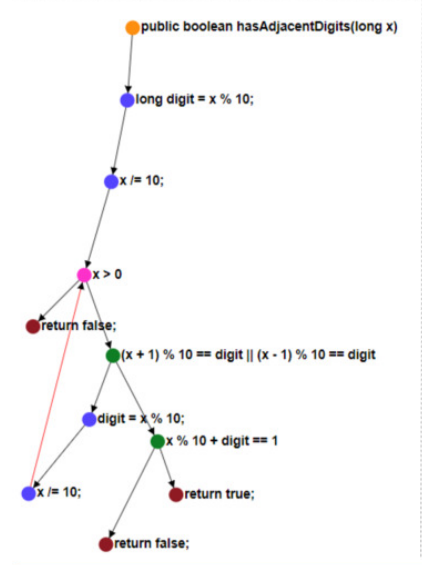
\includegraphics[width=7cm]{flow.png}
                \caption{制御フローグラフ}
                \label{fig:flow}
            \end{figure}

            制御フローグラフは、構造を視覚的に表現できる手法として
            プログラム分析やコンパイラ設計の分野で利用されている。
            コードの流れを直感的に把握できるため、デバッグや最適化、プログラム検証などで
            活用されている。教育の分野でも、学生がコードの流れを理解しやすくするための
            ツールとして注目されている。制御フローグラフによるフィードバックを与えることで、
            学生がよりシンプルで効率的なコードに改善でき、その後の課題で
            コーディングスキルや自己修正能力が向上したことが示されている。
            このことから、視覚的フィードバックを提供することで学生がコードの改善点をより
            理解しやすくなることが考えられる。しかし視覚的フィードバックだけでは学習者が
            それを見てどのようにコードを改善していくかの方針を考えることが困難な場合が
            あるため、具体的な改善方針が含まれるフィードバックを組み合わせる必要がある。

        \section{Webベースシステムの利点}
        本研究で開発したシステムは、Webページを通じてソースコードを送信し、
        解析結果をその場で表示するWebベースのアプローチを採用している。
        Webベースシステムにすることにより、利用者に対して以下のような
        利便性を提供できる。

        \begin{itemize}
           \item システムのインストールや初期設定が不要
           \item インターネット環境があれば、どのデバイスからでもアクセス可能
           \item 常に最新のシステム機能を利用できるため、手動でのアップデートが不要
        \end{itemize}

        また、開発者側にも以下のような利点が考えられる。

        \begin{itemize}
           \item システムのインストール方法やセットアップ手順の説明が不要
           \item ソフトウェアの改善や不具合修正が迅速に反映できるため、ユーザーへの対応が容易
        \end{itemize}

        これにより、システム導入に関する障壁が大幅に減少し、どんな学習者でも手軽に
        利用できる環境を整えることができる。特に技術的な設定が不要なため、利用者は
        煩わしさを感じることなくシステムを活用することができる点が大きな利点である。

        \section{静的解析の利点}
        本研究のシステムでは、ソースコードに対して静的解析を実施する。静的解析とは、
        ソフトウェアを実行せずにソースコードを解析する手法であり、実行時に
        問題を発見する動的解析とは異なる。静的解析を利用することにより、
        コードの記述段階でエラーを早期に発見でき、実行前に改善を加えることが
        可能となる。さらに、静的解析は学習者がインデント等のコードの品質を高めることに
        繋げるための支援にもなり、コードの整合性や可読性の向上にも貢献する。
        これによってコードの誤読や理解の誤りを防ぐことができ、
        予期しないバグやエラーの修正も効率的に行えるメリットがある。

        \section{本研究に求められること}
        これらの点を踏まえて、本システムに求められる要件は以下のとおりである。
        \begin{itemize}
            \item 初学者向けの静的解析を行うことができる
            \item 学習者に即座にフィードバックを行うことができる
            \item コードの流れの理解を支援することができる
            \item 調査項目の拡張性が期待できる
            \item Webベースのシステムである
        \end{itemize}
        プログラミング初学者が、自身のソースコードのどの部分に問題があり、
        何が原因でエラーになっているのか、また修正方法について理解し
        判断できるようにするため、初学者が直面しやすいエラーに対応した
        ソースコード解析を行い、即座にフィードバックを提供するシステムが
        求められる。このシステムは、学習効率を向上させるだけでなく、
        学習者がコードの流れや構造を正しく理解できるよう支援することを目指す。
        さらに、運用の中で新しいエラーや課題が発生した際、
        それらを柔軟に追加・拡張できるようにシステムを実装することで、
        システムの対応範囲を広げ、学習者の多様なニーズに応えることが
        可能となる。これにより、利用者が増加し、より多くの学習者に
        貢献することが期待される。学習者が気軽に利用できるように、
        システムをWebベースで実装することで、アクセス性を向上させることが必要である。

        \section{章構成}
        本論文の構成は以下のようになっている。
        第2章で本システムを実装するにあたって使用した技術について説明する。
        第3章では実装したシステムについて述べる。
        第4章では本システムの試用実験と評価について述べる。
        第5章で本論文のまとめと課題点について述べる。

    \chapter{使用技術}
    ここでは本システムで使用した技術について説明する。

        \section{Haskell}

            \subsection{Haskellとは}
            Haskellは、関数型プログラミング言語の一つであり、
            計算や処理を関数の組み合わせとして数学的に表現し、
            記述することを特徴としている。この言語は、記号論理学者である
            Haskell Brooks Curry氏の名前にちなんで名付けられている。
            現在、Haskellの主な処理系としては、
            GHC (Glasgow Haskell Compiler) が広く使用されている。
      
            \subsection{Haskellの特徴}
            Haskellは関数型言語に特有の機能を数多く備えており、
            パターンマッチングや型推論などの特徴を持っている。
            これらの機能や技術を組み合わせることで、命令型言語に比べて
            Haskellはより簡潔かつ効率的にコードを記述できる場合が多く、
            特に構文解析やデータ処理の分野でその強みを発揮する。
            以下にHaskellの代表的な特徴をいくつか示す。
            \begin{itemize}
                % \item 参照透過性
            
                % C言語やJavaなどの命令型言語では、課題解決のために
                % 命令や手続きを組み合わせて記述する。このアプローチでは、
                % システムの状態が命令の実行によって変化するため、
                % 複数の処理が同じ変数を参照している場合、
                % 予期しない結果が生じることがある。このような現象は
                % 「副作用」と呼ばれ、デバッグやメンテナンスの複雑化を招く
                % 要因となる。一方、Haskellを含む関数型言語では、
                % プログラムの目的に沿った関数を定義することで記述を進め、
                % 副作用を極力排除する設計思想が採用されている。
                % 特にHaskellは「参照透過性」という性質を持ち、
                % 同じ引数で呼び出した関数が常に同じ結果を返す。
                % この数学的な特徴により、プログラムの挙動が予測可能となり、
                % 安全性と信頼性が向上する。また、参照透過性は関数のテストや
                % 再利用を容易にし、大規模なコードベースにおいても
                % 品質を維持する重要な要素となる。

                % \item 遅延評価
            
                % 一般的なプログラミング言語では、関数を呼び出す際、
                % 引数が事前に評価され、その結果が関数に渡される
                % 「正格評価」が採用されている。一方、Haskellでは
                % 「遅延評価」という特性があり、引数の値が実際に必要に
                % なるまで評価が行われない。この特性は関数の引数だけでなく、
                % 変数の値を参照する際にも適用される。遅延評価の利点として、
                % 無限リストのような無限データ構造を扱える点が挙げられる。
                % 例えば、以下のコードでは無限リストを生成し、
                % 必要な部分だけを取り出して計算を行うことができる。

                % \begin{lstlisting}
                % take 5 [1..]
                % -- 結果: [1, 2, 3, 4, 5]
                % \end{lstlisting}

                % この仕組みにより、必要最小限の計算だけが実行されるため、
                % 計算効率が向上し、プログラムの柔軟性を高めることができる。
                % 例えば条件分岐で実際に使用されない計算を
                % スキップすることができる。ただし、遅延評価には注意点も
                % ある。計算が後回しにされるため、大規模なデータ構造を
                % 扱う場合にメモリ使用量が予想外に増加するリスクがある。
                % そのため、遅延評価の特性を理解し、適切に設計することが重要である。

                \item パターンマッチング
                
                Haskellでは、関数定義においてパターンマッチを
                利用することで、入力引数に応じた条件分岐を簡潔に記述できる。
                この機能はコードの可読性を向上させるとともに、
                安全で明確なプログラムの構築を可能にする。
                関数呼び出し時には関数定義内のパターンが上から順に評価され、
                最初にマッチしたパターンに対応する処理が実行される。
                マッチするパターンが存在しない場合にはエラーが発生する。
                以下に階乗を計算する関数の例を示す。

                \begin{lstlisting}
                fact 0 = 1
                fact n = n * fact (n - 1)
                \end{lstlisting}

                この関数は、引数が0の場合に1を返す。引数が0以外の
                任意の値の場合はnに値が束縛され、再帰的に
                fact (n - 1) を呼び出して計算が進行する。
                パターンマッチングを用いることで、複雑な条件分岐を簡潔に
                記述することができる。この特徴によりコード全体の
                可読性が向上し、結果として保守性も高まる。
                特に条件分岐が多い場合でも分かりやすい記述が可能であり、
                プログラムの設計や実装が容易になる。さらに、
                パターンマッチングはプログラムの安全性を向上させる役割も果たす。
                未対応のケースが存在する場合、コンパイル時に警告が表示されるため、
                プログラマは問題を事前に発見しやすくなる。
                ワイルドカードなどを活用することで、
                すべてのケースを網羅的に記述することが可能となり、
                プログラムの信頼性が高まる。このように、
                パターンマッチングは効率的で安全なプログラミングを支える重要な機能である。

                \item 型推論
            
                Haskellの型推論機能は、プログラマに対して
                静的型付けの利点を提供しつつ、
                コードの簡潔さと可読性を高めるものである。
                静的型付けはコンパイル時にエラーを事前に発見できるという
                メリットを持つ一方で、データ型を明示的に指定する必要があり、
                プログラムの複雑さや冗長さを招く可能性がある。
                一方、動的型付けではデータ型を指定する手間が省けるが、
                エラーが実行時まで発見されないというデメリットを伴う。
                Haskellの型推論は、これらの両者の短所を補完するよう
                設計されている。型推論により、プログラマはデータ型を
                明示的に指定する必要がなく、与えられたコードから
                コンパイラが自動的に型を推測し、適切に判断する。
                これによりプログラムの記述は簡潔になり、
                複雑な型指定による冗長さを回避できる。
                さらに型推論の機能は、コンパイル時にコードの正確性を
                保証する点で非常に有効である。
                明示的な型指定が不要でありながら、
                静的型付けと同様にコンパイル時にエラーを検出できるため、
                コードの安全性を確保し、エラーの発生を抑えることが可能となる。
                これによりHaskellのプログラミング環境は、
                簡潔なコード記述とエラー抑制の両立を実現している。

                % \item モナド
                
                % モナドは、Haskellにおいてプログラムの副作用を安全かつ
                % 体系的に扱うための枠組みである。ここでいう副作用とは、
                % 状態の変更を伴う破壊的代入や入出力操作など、
                % プログラミングにおける一般的な副作用を指す。
                % モナドは、これら副作用を伴う処理を共通の構造を通じて
                % 抽象化し、その構造に基づいた演算子を用いることで一貫して
                % 扱うことを可能にする。これにより、副作用を安全に
                % 管理するための強力なツールを提供している。
                % 特にHaskellで頻繁に使用されるモナドの一つがIOモナドであり、
                % 主に入出力操作に関連する役割を担う。IOモナドを用いることで、
                % 標準入力や標準出力といった外部とのやり取りを安全に
                % 記述することが可能である。以下に、IOモナドを用いた
                % プログラムの例を示す。

                % \begin{lstlisting}
                % main :: IO ()
                % main = do
                %             line <- getLine
                %             putStrLn line
                % \end{lstlisting}

                % このコードでは、getLineによって標準入力から文字列を取得し、
                % それを変数lineに束縛している。その後、putStrLn関数を用いて、
                % 取得した文字列を標準出力に表示する。putStrLnは文字列String型
                % を引数として受け取り、標準出力への表示を行うIOアクションを返す
                % 関数である。このように、IOモナドを用いることで、
                % 外部とのやり取りを明確に区別しながら副作用を管理することができる。

            \end{itemize}
            % Haskellにはこれらのような特徴があり、構文解析やデータ処理では、
            % 抽象構文木の操作や再帰的な処理が頻繁に求められるが、これらは
            % Haskellの強みであるパターンマッチングやGenericsなどを
            % 活用することで効率的かつ安全に実現できる。

            \subsection{language-c-quote}
            language-c-quote \cite{7}はHaskellのライブラリであり、
            一般的なC言語のパーサを提供している。
            language-c-quoteは構文解析の結果が扱いやすいため、
            新しく調査項目を増やす際に容易にプログラムを
            追加することができると考え本システムの構文解析に用いている。
            特に、構文解析の結果がHaskellのデータ型としてそのまま表現されるため、
            型安全性を活かしつつ追加処理の実装や拡張が効率的に行える点、
            実装コストが低く、C言語の複雑な構文規則にも対応済みである点が利点である。
            以下に実際にC言語のソースコードを解析した結果を載せる。
            その解析結果から調査したい構文等を抜き出し真偽を確かめている。
            \begin{figure}[h]
                \centering
                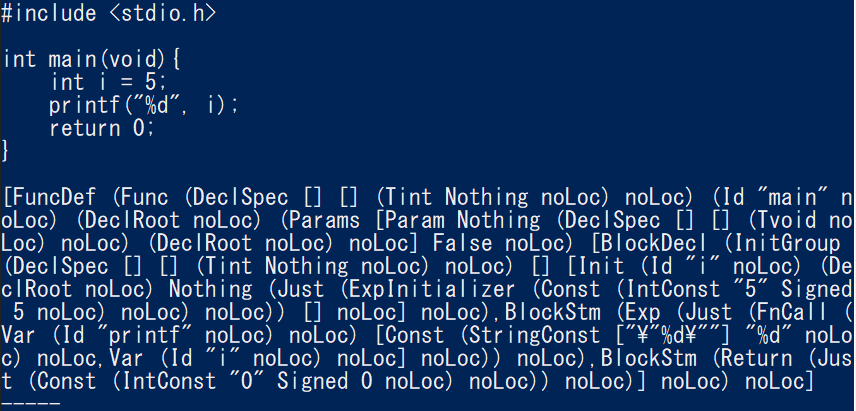
\includegraphics[width=15cm]{lcq.png}
                \caption{language-c-quoteによるソースコードの解析結果}
                \label{fig:lcq}
            \end{figure}

            \subsection{Generics}
            HaskellにおけるGenerics \cite{8}は、型に依存しない汎用的なプログラミングを
            可能にする機能であり、Haskellの抽象性や型システムの強力さを活用した
            仕組みである。型ごとに個別のコードを書くのではなく、
            汎用的な操作を記述し、データ型全般に適用できるようにすることを
            目的としている。
            その中でも、Scrap Your Boilerplate (SYB) \cite{9}は、
            特に複雑なデータ構造を扱う際に発生しがちな冗長なコードを
            削減することを目的としている。SYBは、再帰的データ構造を
            簡潔に操作するためのツールを提供し、データ操作の記述を効率化するものである。
            以下に実際にGenericsを活用したコードの例を挙げる。

            \begin{lstlisting}
                {-# LANGUAGE DeriveDataTypeable #-}
                import Data.Generics

                -- データ型の定義
                data Expr = Val Int
                        | Add Expr Expr
                        | Mul Expr Expr
                        deriving (Show, Data, Typeable)

                -- 値を2倍する
                double :: Expr -> Expr
                double (Val n) = Val (n * 2)
                double x       = x

                -- 任意の型に対する操作を適用するための関数
                apply :: Data a => (a -> a) -> a -> a
                apply f = everywhere (mkT f)

                -- 2倍する関数をExprに適用
                doubleValues :: Expr -> Expr
                doubleValues = apply double

                expr :: Expr
                expr = Add (Val 1) (Mul (Val 2) (Val 3))

                main :: IO ()
                main = print $ doubleValues expr

                -- 出力結果 Add (Val 2) (Mul (Val 4) (Val 6))
                                                
            \end{lstlisting}

            everywhereとmkTを活用することで、特定のデータ型に依存せず任意の操作を
            データ型全体に適用することが可能となっている。
            これによりデータ型ごとに異なる処理を記述する必要がなく、
            コードが簡潔で再利用可能なものとなる。
            関数applyにより、Exprのような再帰的なデータ型に対して
            データ構造全体にわたる再帰的な操作を行うことができる。
            再帰的にデータ構造をたどりながら処理を行うため、
            Expr型の全ての要素であるVal、Add、Mulに対して同じ操作が適用され、
            出力結果では全ての値に2倍する関数が適用されていることが分かる。
            さらに、Expr型に新しく Sub Expr Expr のような構造を追加した場合でも、
            他の関数はそのままで同様に機能し、Subの値に対しても
            再帰的に処理が適用されることとなる。
            この特徴により、コードの変更箇所を少なく容易に新しい型の追加や
            変更が行え、拡張性が期待される。
            
        Haskellにはこれらのような特徴があり、構文解析やデータ処理では
        抽象構文木の操作や再帰的な処理が頻繁に求められるが、これらは
        Haskellの強みであるパターンマッチングやGenericsなどを
        活用することで効率的かつ安全に実現できる。

        \section{Haskell関連技術}
            \subsection{GHCup}  
            GHCup \cite{10} は、GHCおよび関連ツールのインストールや
            バージョン管理を行うためのツールである。  
            関連ツールには、CabalやHLSなどが含まれる。  
            GHCupは複数のバージョンを同時に管理できるため、
            最新バージョンのGHCを利用したい場合や、古いバージョンのGHCでしか
            動作しないツールを使用したい場合に柔軟に対応できる。  
            また、`ghcup list`コマンドを使用することで、
            インストールされている内容を確認することが可能である。

            \subsection{Cabal}  
            Cabal \cite{11} は、Haskellのライブラリやプログラムをビルド及び
            パッケージ化するためのシステムである。  
            パッケージの作成者および配布者がアプリケーションを移植可能な形で
            簡単に構築できるよう、共通のインターフェースが提供されている。  
            本システムでは、プロジェクトの作成や必要なライブラリ及び
            パッケージのインストールにCabalを利用している。

            \subsection{HLS}
            HLS (Haskell Language Server) \cite{12} は、Haskellプログラミングを
            支援するために Language Server Protocol (LSP) を実装したサーバである。  
            HLSはVS CodeやEmacsといったLSP対応エディタと組み合わせることで、
            警告やエラーのハイライト、コード補完、マウスオーバーによる型や
            ドキュメントの表示、定義へのジャンプなどの便利な機能を提供する。

            \subsection{Wai}  
            Wai \cite{13} は、WebアプリケーションとWebサーバ間の
            通信プロトコルを提供するための Haskell ライブラリである。  
            Wai を使用することで、Webブラウザ上の入出力とサーバ側の
            Haskellシステムを接続できる。

            \subsection{Warp}
            Warp \cite{14} は、Waiを処理するための高速かつ軽量なHTTPサーバである。  
            本システムでは、Haskellプログラム内でWarpを利用してサーバを構築し、
            ブラウザを通じてアクセスすることでシステムを実行可能としている。
            以下にWaiとWarpを用いて簡単なWebアプリケーションを作成する方法を載せる (図\ref{fig:warp})。

            \begin{figure}[h]
                \includegraphics[width=15cm]{wai.png}
                \caption{Wai、Warpによるアプリケーション作成}
                \label{fig:warp}
            \end{figure}

             これをbuildしてrunし、localhost:8080を開くとHelloが表示されている。

            
        \section{ブラウザ上での出力に関する技術}
            \subsection{Mermaid.js}
            Mermaid.js \cite{15}は、テキストベースでフローチャートやシーケンス図、
            ガントチャートなどのダイアグラムを記述・生成できるJavaScriptライブラリである。
            Markdown形式のようなシンプルな構文でダイアグラムを定義できるため、
            プログラムやドキュメント内での利用が容易であり、視覚的な情報表現を手軽に実現する。
            本システムでは、Mermaid.jsを利用してC言語の制御構文を視覚化し、
            初学者がコードの流れを直感的に理解できるように設計した。
            Mermaid.jsを採用した主な理由は以下の通りである。
            \begin{itemize}
                \item コードを直接グラフ構造に変換するためのシンプルな文法を持つ。
                \item ブラウザ上での即時描画に対応し、Webベースシステムとの親和性が高い。
                \item 制御フローやロジックをフローチャート形式で分かりやすく表示可能である。
            \end{itemize}
            以下はMermaid.jsによるフローチャート生成の例である(図\ref{mermaid})。
            \begin{lstlisting}
                graph LR
                A --> B
                B -- 条件が真 --> C
                B -- 条件が偽 --> D
                C --> E
                D --> E
            \end{lstlisting}
            \begin{figure}[h]
                \centering
                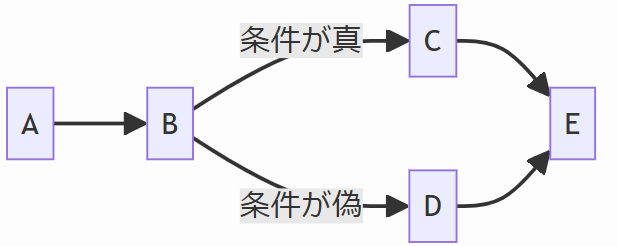
\includegraphics[width=13cm]{mermaid.png}
                \caption{Mermaid.jsによるフローチャート生成}
                \label{fig:mermaid}
            \end{figure}

            このような視覚化により、初学者がコードの論理構造を容易に理解できる環境を提供している。

            \subsection{CodeMirror}
            CodeMirror \cite{16}は、ブラウザ上で動作するコードエディタで、
            複数のプログラミング言語に対応しており、シンタックスハイライト、
            オートコンプリート、エラー表示などの機能を提供する。
            本システムではCodeMirrorを活用して、学習者が入力したコードに
            対してエラー箇所をハイライトすることで直感的に
            把握できるようにするために利用している。
            エラー箇所ハイライト機能はコードの文法エラーや
            警告が発生した位置を視覚的に示すことができる。
            エラーが発生した行に色付けを行うことで、
            誤った部分を強調し効率的に学習支援を行う。
            これにより、学習者は自分のコードの問題をすぐに認識し、
            修正を行うことができる。

    \chapter{システムの実装}
    ここでは本システムについて実際の実行画面を踏まえて詳細に述べる。
        \section{システムの概要}
        本システムは、主にプログラミング講義で学習者が提出する、
        課題に対して記述されたコードを対象とし、
        そのコードを解析して学習者にフィードバックを提供することを目的として構築する。
        学習者が書いたソースコードを構文解析してデータを読み取り、
        コードの構造を自動的に検出し、ある構造の特定や指摘に利用する。
        その結果をもとに、どこに問題があるのか、
        またどのように改善すればよいのか等の指摘やフィードバックを行う。
        対象とする言語は、香川大学創造工学部情報システム・セキュリティコースと
        人工知能・通信ネットワークコースで初めに学習するC言語のソースコードとする。
        本研究のシステムはHaskellのプロジェクトであり、
        WaiとWarpを用いることでWebベースでの
        システム構築を行っている。
        本システムの開発環境としては、GHCup 0.1.18.0、
        Cabal 3.6.2.0、HLS 1.8.0.0、GHC 8.10.7を用いている。
        Waiの機能を用い、URLによるルーティング機能が付いた
        サーバを立ち上げている。
        実装は以下のようになっている。
        \begin{lstlisting}
            main :: IO ()
            main = do
                Warp.run 8080 router
            
            router :: Wai.Application
            router req =
                case Wai.pathInfo req of
                [] -> app req
                ["compare"] -> compare req
                ["teacher"] -> teacher req
                _ -> notapp req
        \end{lstlisting}
        ここで、Warpによりポート8080上にHTTPサーバを起動しており、
        Wai.pathInfo reqを使用してリクエストパスを取得し、
        その内容に応じた処理を行っている。
        ルートパスなら関数app、/compareにアクセスすれば
        関数compareにリクエストを渡し処理が行われる。
        
        システムの全体図としては以下の図\ref{fig:system}のようになっている。

        \begin{figure}[h]
            \centering
            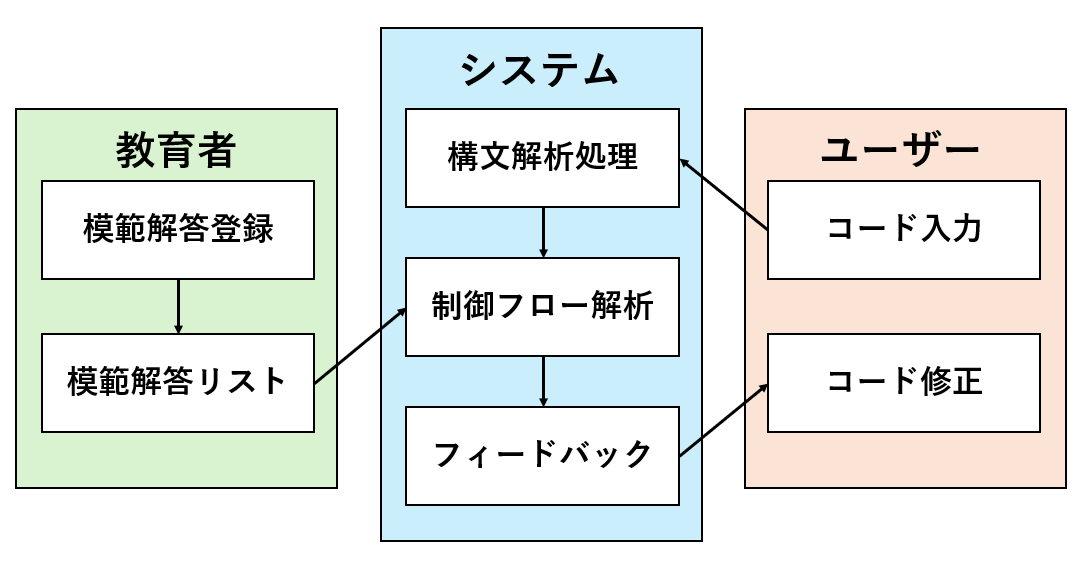
\includegraphics[width=13cm]{system.png}
            \caption{システム全体図}
            \label{fig:system}
        \end{figure}

        システムの全体の流れは以下のようになっている。
        まず学習者がブラウザ上で自分の記述したソースコードを入力し、
        それをシステムが受け取り構文解析を行う。
        解析によりコードの構造を自動的に検出し、解析結果とフィードバックを即時に
        ブラウザ上に出力する。フィードバックがすぐに与えられることで学習者は
        その場でコードの修正に取り組むことができる。また、Webアプリケーションとして
        実装することでインストールなどの手間を省き、学習者にとって利用しやすく、
        自己学習の効率を向上させることができるシステムを構築する。
        フィードバックは、視覚的な情報とテキストメッセージを組み合わせて提供される。
        制御フローの視覚的フィードバックでは、分岐やループといった
        コード内の複雑な部分を直感的に把握できるようにする。
        テキストメッセージでは、具体的にどの部分に問題があるのか、
        どう改善すればよいのかのフィードバックを提供する。
        これにより具体的な改善方針を学習者に与え、
        初学者でも理解しやすく、改善を行いやすいフィードバックを目指す。
        また本システムではプログラミング教育における利用を考慮し、
        学習者が課題に対して提出するために記述したコードと
        模範解答の解析結果を比較する機能を提供する。
        教育者が模範解答のコードを登録することで、
        学習者は登録されている模範解答のファイル名に応じた
        個別の解析ページにアクセスすることができ、
        模範解答と自身のコードの解析結果である制御フローを比較することができる。
        この制御フローの比較により、自身のコードの複雑な構造や冗長な部分を
        視覚的に理解することができ、より簡潔で効率的なプログラムを
        記述することができるようになる。

        \section{システムの入手方法や実行}
        本システムは https://github.com/Kagawa-Laboratory/Haslan から
        次のようなコマンドで入手することができる。
        \begin{lstlisting}
            git clone https://github.com/Kagawa-Laboratory/Haslan.git
        \end{lstlisting}

        本システムは主に以下のようなファイルからなる(表\ref{table:file})。
        \begin{table}[h]
            \caption{システムのファイル構成}
            \label{table:file}
            \centering
            \begin{tabular}{ccc}
              \hline
              フォルダ/ファイル名     & 主な役割                              \\
              \hline
              app    &   システムの実行ファイルMain.hsを配置   \\
              \hline
              src    & Main.hsで利用される主要なライブラリが記述されたMyLib.hsを配置        \\
              \hline
              static    & システムで扱うWebページの設定である.htmlファイルを配置                                \\
              \hline
              Dockerfile    & Dockerコンテナの作成情報が記載                 \\
              \hline
              start-haskell.cabal    & システムのビルド情報、依存関係等の記載          \\
              \hline 
            \end{tabular}
        \end{table}

        本システムは以下のコマンドでビルド、実行できる。
        \begin{lstlisting}
            cabal build all

            cabal run start-haskell
        \end{lstlisting}

        本システムはwodenにDockerコンテナとして立ち上げられており、
        ymirを使用してリバースプロキシが行われている。
        wodenとymirはそれぞれ香川研究室に設置されたサーバである。
        学外からのリクエストはymirにより学内サーバであるwodenに
        渡されるため、学外からもサーバへのアクセスが可能である。

        Dockerfileの内容を以下に示す。
        \begin{lstlisting}
            FROM library/ubuntu:22.04

            RUN mkdir haslan
            COPY dist-newstyle/build/x86_64-linux/ghc-9.2.8/start-haskell-0.1.0.0/x/start-haskell/build/start-haskell/start-haskell haslan/
            COPY static haslan/

            RUN apt-get update && apt-get install -y socat

            RUN mkdir -p /tmp/haslan
            RUN chmod a+w /tmp/haslan

            RUN echo "#!/bin/bash" > start.sh
            RUN echo "./haslan/start-haskell &" >> start.sh
            RUN echo "exec socat UNIX-LISTEN:/tmp/haslan/haslan.unixsocket,fork,user=www-data,reuseaddr TCP4:127.0.0.1:8080" >> start.sh
            RUN chmod a+x start.sh

            VOLUME ["/tmp/haslan"]
            CMD ["./start.sh"]
        \end{lstlisting}

        \section{ソースコードの解析}
        解析にはプログラミング言語Haskellを利用する。
        Haskellは、純粋関数型プログラミングの特徴を持ち、
        関数の再利用や組み合わせによってシステム全体を柔軟に構築することに優れている点や、
        高い抽象化能力により、複雑な解析結果もシンプルに扱うことができる点がある。
        それらを利用することにより、特に、既存の関数やモジュールを組み合わせることで、
        新しい機能を柔軟に拡張できる点が強みとなる。
        またHaskellは強力な静的型システムによりコンパイル時に型の安全を確認できるため、
        機能の拡張に伴うリスクを最小限に抑え、堅牢で信頼性の高い解析機能を
        実現することができる。
        本システムでは以下のような処理を行う。
        \begin{enumerate}
            \item ソースコードの読み取り\\
            C言語のソースコードを文字列としてプログラムに入力する。
            \item 構文解析\\
            Haskellのライブラリlanguage-c-quoteを利用して、
            C言語のコードを解析し、構造の抽出・特定を行う。  
            \item 解析結果の視覚化\\
            構文解析の結果をフローチャートのような形式で視覚化するため、
            解析結果をMermaid形式に変換し、ブラウザ上で描画する。  
        \end{enumerate}

        Haskellのライブラリであるlanguage-c-quoteを用いた構文解析について、詳しく述べる。
        まず、以下のような関数を Haskell で作成する。

        \begin{lstlisting}
        import Language.C
        import Data.ByteString.UTF8 as UTF8 (fromString)

        parseProg :: String -> Either SomeException [Definition]
        parseProg str = parse [C11] [] parseUnit (UTF8.fromString str) Nothing
        \end{lstlisting}

        この関数parseProgでは、引数strとして
        C言語ソースコードの文字列を渡すことで構文解析が行われる。
        実際に次のような簡単なC言語プログラムを入力した場合を示す。

        \begin{lstlisting}
        #include <stdio.h>
            
        int main(void){
            int i = 5;
            if (i == 5) {
                printf("%d", i);
            }
            return 0;
        }
        \end{lstlisting}

        この文字列を関数parseProgに渡すと、構文解析が行われ、
        コードの各部分がどのような構造になっているかが出力される。
        以下は、解析結果を出力したものである。

        \begin{figure}[h]
            \centering
            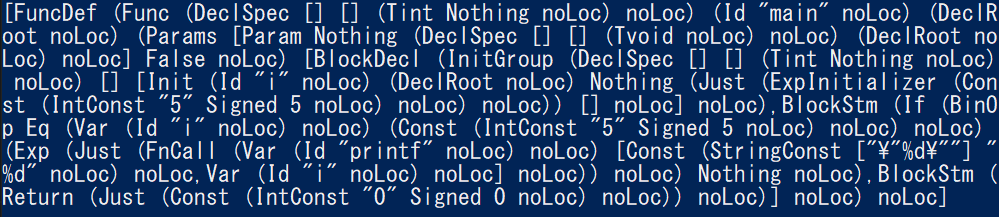
\includegraphics[width=13cm]{lcq1.png}
            \caption{language-c-quoteで解析した結果}
            \label{fig:lcq1}
        \end{figure}

        上記の解析結果から、特定の構文、たとえばif文やprintfの部分を見つけ出し、
        その中身を確認することができる。  
        たとえば、`if (i == 5)` の部分は次のように解析されている。

        \begin{lstlisting}
            BinOp Eq (Var (Id "i" noLoc) noLoc) (Const (IntConst "5" Signed 5 noLoc) noLoc) noLoc
        \end{lstlisting}

        ここでは、以下のように解析結果を読み取ることができる。

        \begin{itemize}
            \item BinOp Eq は「等号演算子(==)」を意味する。
            \item Var (Id "i" ...) は変数 i を表す。
            \item Const (IntConst "5" ...) は定数5を表す。
        \end{itemize}

        つまり、元の C 言語コードで if (i == 5) と書かれていた条件式が、
        このように分解されている。

        同様に、\verb|printf("%d", i)|の部分は次のように解析される。

        \begin{lstlisting}
            Exp (Just (FnCall (Var (Id "printf" noLoc) noLoc) [Const (StringConst ["%d"] "%d" noLoc) noLoc, Var (Id "i" noLoc) noLoc] noLoc)) noLoc
        \end{lstlisting}

        ここでは、

        \begin{itemize}
            \item FnCall が関数呼び出しを意味する。
            \item Var (Id "printf" ...) は printf関数を表す。
            \item Const (StringConst [\verb|"%d"|] ...) はフォーマット指定子 \verb|%d|を表す。
            \item Var (Id "i" ...) は変数iを表す。
        \end{itemize}

        これに基づき、printfの情報を抽出し、条件式やパラメータのミスを検出する。
        本システムでは、上記の方法に基づいて他の構文についても
        同様の処理が可能である。
        % language-c-quoteで解析された結果を適切に読み取るためには、
        % 解析結果に含まれる複数のデータ型とその構成を理解することが
        % 重要である。データ型の詳細はLanguage.C.Syntax \cite{17}に
        % 記載されており、上記のように解析結果を参照しながら
        % 目的の構文を特定していく。

        また、解析された結果に関数を適用する場合は、以下のように処理を行う。
        \begin{lstlisting}
            countControl :: [Definition] -> [Int]
            countControl = everything (++) ([] `mkQ` countControlStm')

            countControlStm :: Stm -> [Int]
            countControlStm (If _ _ Nothing _)  = [1]
            countControlStm (If _ _ (Just _) _) = [2]
            countControlStm (For _ _ _ _ _)     = [3]
            countControlStm (Switch _ _ _)      = [4]
            countControlStm (While _ _ _)       = [5]
            countControlStm (DoWhile _ _ _)     = [6]
            countControlStm _                   = []

            let intlist = countControl defs
        \end{lstlisting}

        関数parseProgによって構文解析された結果であるdefsの型は
        [Definition]となっており、解析された結果に対してevrythingやmkQといった
        Generics技術を用いて再帰的に処理を行っている。
        関数countControlStmではパターンマッチングを利用し、
        解析結果の中から制御構造のパターンを抜き出して
        それぞれに対応した整数を返却する処理が行われる。
        再帰的に処理が行われるため、ネストが深くなっても
        値を参照することが可能であり、入れ子構造のような
        複雑な構造であってもコードの解析結果全体に対して
        関数を適用することができる。
        このような形で解析結果に対する調査を行う関数を記述し、
        Generics技術やパターンマッチングを活用することで
        効率的なデータ処理を実装することが可能である。

        language-c-quoteで解析された結果を適切に読み取るためには、
        解析結果に含まれる複数のデータ型とその構成を理解することが
        重要である。データ型の詳細はLanguage.C.Syntax \cite{17}に
        記載されており、上記のように解析結果を参照しながら
        目的の構文や形を特定していく。
        Language.C.Syntaxの構造を理解し、解析結果への処理を行う
        コードを記述することで、新たな調査項目への対応が容易となる。
        この点において、システムの拡張性が保証されているといえる。

        \section{筆者の先行研究}
        本システムのエラー検出機能は、筆者が過去に開発したWebアプリケーションシステムを
        活用している。この過去のシステムでは、プログラミング初学者が陥りやすい構文的なミスや
        論理的な誤りを検出し、学習支援を行うことを目的としており、その詳細については
        先行研究 \cite{18}で述べている。
        そのシステムで検出できるエラー項目は以下のとおりである。
        \begin{itemize}
            \item インデントのミス
            \item printfの変数の数が間違っているミス
            \item scanfの変数の数が間違っているミス
            \item if文の条件式が関係演算子ではなく代入式になっているミス
            \item 関数名が他の関数と重複しているミス
            \item 返却値がint型の関数にreturnが記述されていないミス
        \end{itemize}
        本研究では、このエラー検出システムを基盤として利用しつつ、
        C言語の制御構文をフローチャートの形で可視化し、コードの流れを
        より理解しやすくなるように改良を加えている。

        \section{解析可能な項目}
        本システムでは制御構文をグラフ上に可視化している。
        対応している制御構文と描画されるグラフの例を示す。

            \subsection{If文}
            \begin{lstlisting}
                #include <stdio.h>

                int main() {
                    int num = 10;
                    if (num > 0) {
                        printf("正の数です。");
                    }
                    return 0;
                }
            \end{lstlisting}

            グラフ上での表示は以下の図\ref{fig:if}のとおりである。

            \begin{figure}[h]
                \centering
                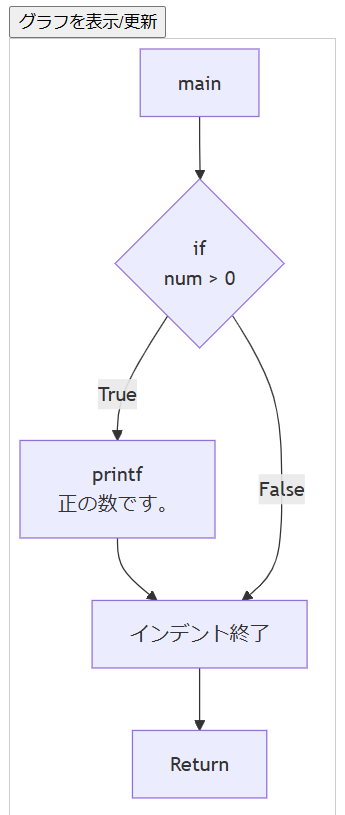
\includegraphics[width=6cm]{if.png}
                \caption{if文の描画例}
                \label{fig:if}
            \end{figure}

            \subsection{For文}
            \begin{lstlisting}
                #include <stdio.h>

                int main() {
                    for (int i = 0; i < 5; i++) {
                        printf("%d", i);
                    }
                    return 0;
                }
            \end{lstlisting}
            グラフ上での表示は以下の図\ref{fig:for}のとおりである。

            \begin{figure}[h]
                \centering
                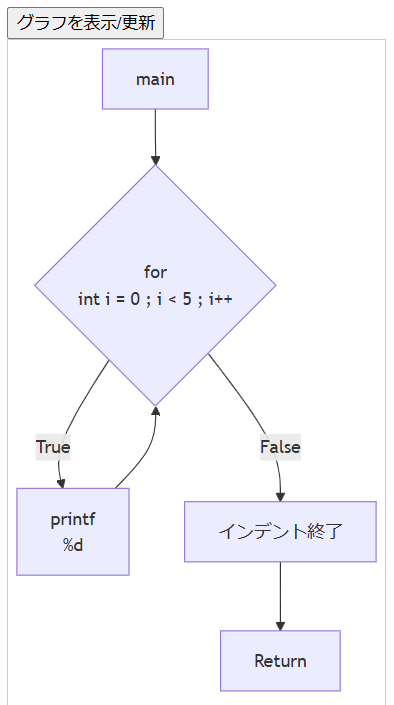
\includegraphics[width=8cm]{for.png}
                \caption{for文の描画例}
                \label{fig:for}
            \end{figure}

            \subsection{While文}
            \begin{lstlisting}
                #include <stdio.h>

                int main() {
                    int i = 0;
                    while (i < 5) {
                        printf("%d", i);
                        i++;
                    }
                    return 0;
                }
            \end{lstlisting}

            グラフ上での表示は以下の図\ref{fig:while}のとおりである。
            
            \begin{figure}[h]
                \centering
                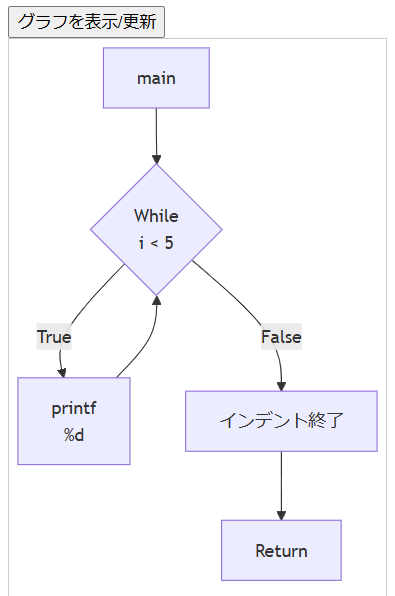
\includegraphics[width=8cm]{while.png}
                \caption{while文の描画例}
                \label{fig:while}
            \end{figure}。

            \subsection{Do-While文}
            \begin{lstlisting}
                #include <stdio.h>

                int main() {
                    int i = 0;
                    do {
                        printf("%d", i);
                        i++;
                    } while (i < 5);
                    return 0;
                }
            \end{lstlisting}

            グラフ上での表示は以下の図\ref{fig:dowhile}のとおりである。

            \begin{figure}[h]
                \centering
                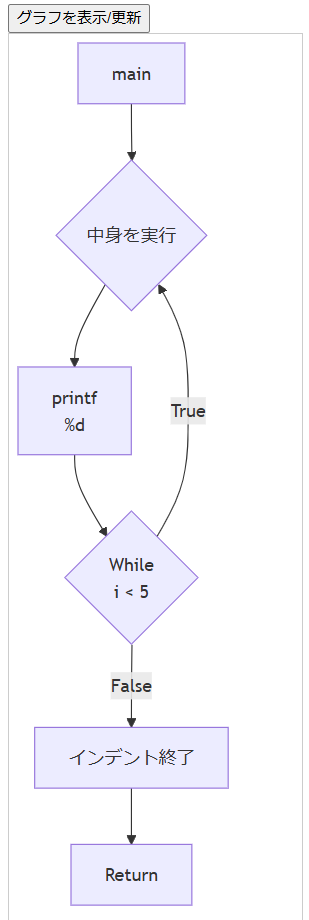
\includegraphics[width=4cm]{dowhile.png}
                \caption{do-while文の描画例}
                \label{fig:dowhile}
            \end{figure}

        \section{システムの実行}
        本システムはWebページにアクセスすることでシステムを利用できる。
        システムページにアクセスすると、入力フォームが表示される(図\ref{fig:systemuse1})。
        
        \begin{figure}[h]
            \centering
            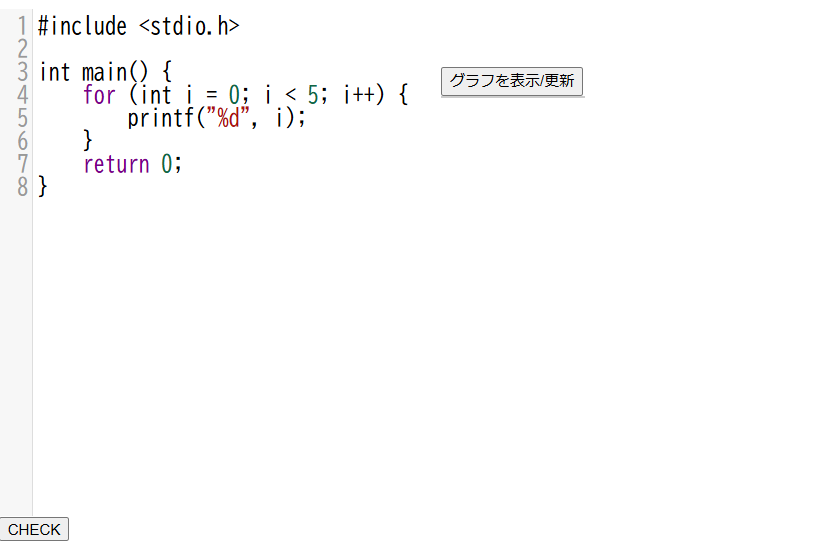
\includegraphics[width=10cm]{systemuse1.png}
            \caption{ソースコード入力画面}
            \label{fig:systemuse1}
        \end{figure}

        表示されているテキストエリアに解析したい
        ソースコードを入力し、CHECKボタンを押すことで
        Haskellプログラムに文字列として
        ソースコードが送信され、構文解析が行われる。
        そして解析した結果とエラーの箇所や内容、
        生成した制御フローグラフの表示が行われる。
        結果表示の際にはエラーがある行番号の色を変更することで強調している。
        実際にソースコードを入力した際の結果表示画面を以下に示す(図\ref{fig:systemuse2})。

        \begin{figure}[h]
            \centering
            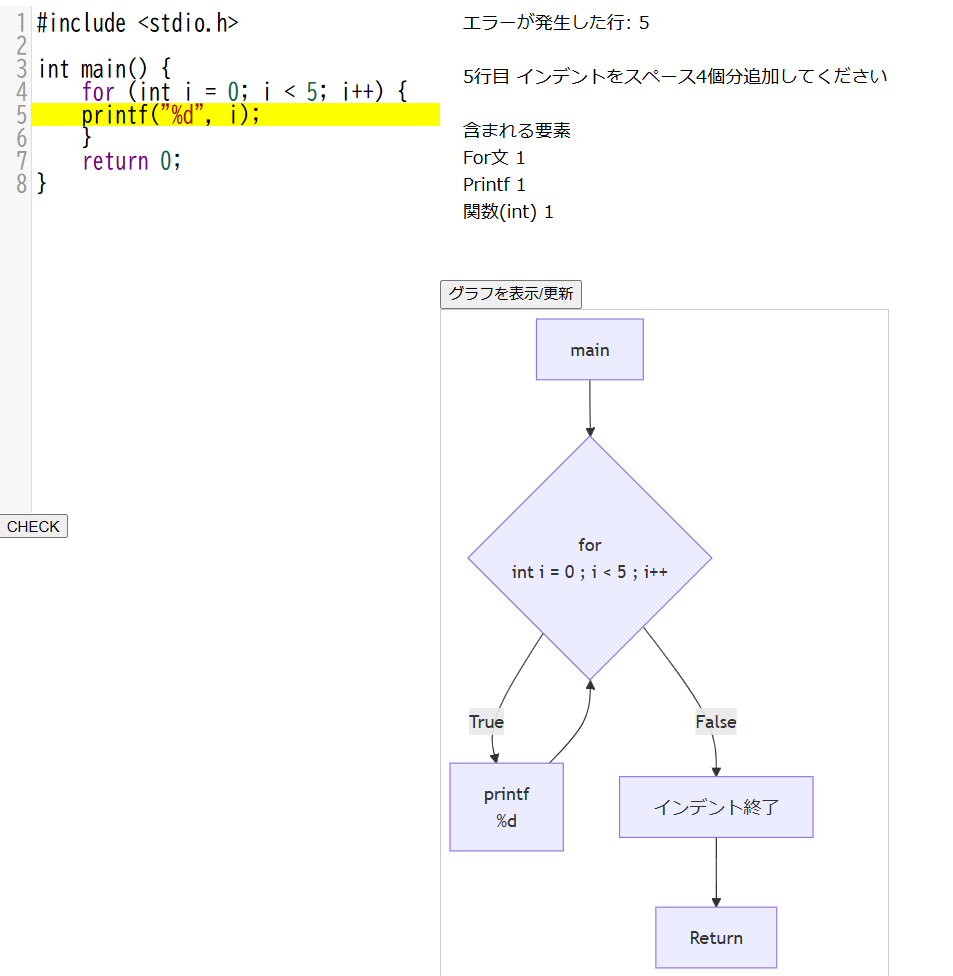
\includegraphics[width=10cm]{systemuse2.png}
            \caption{解析結果表示画面}
            \label{fig:systemuse2}
        \end{figure}

        解析結果の表示画面では特に初学者がソースコードのエラーを
        修正できるように分かりやすくエラー内容を表示することを意識している。
        エラーがある行はCodeMirrorを利用しハイライトすることで
        一目で間違っている行を理解することができる。
        通常のコンパイラでは文字情報でしかエラー内容が示されていないため、
        視覚的にエラー箇所を理解することができない。
        また、画面右側では生じているエラーの内容について行番号と共に記している。
        エラーによっては修正するために何を行えば良いかの提案もしており、
        表示を見てすぐにエラーの修正を行うことができる。
        さらに解析した結果コードに含まれている特定の要素の数を
        表示している。課題によってはfor文を必ず使用することといった条件が
        設定されることも考えられるため、自身のコードに含まれる要素を
        確認することができることで正確な解答を記述することに繋がる。
        解析を行うことでコードのグラフを表示することが可能となり、
        描画されたグラフを確認することでコードの制御構造による流れを
        可視化し、学習者の理解を促進させる支援を行う。
        プログラミング講義での活用を考慮し本システムでは通常の解析だけではなく、
        模範解答との比較機能を実装している。
        教育者が模範解答をシステムに登録することで、
        利用者は模範解答のリストを参照することができ、
        それぞれの課題に対応した解析ページにアクセスすることができる。
        そこで自身のコードと模範解答コードの制御フローグラフを
        比較できるようになっており、自身のコードをより簡潔で
        効率的なものとするための支援を提供する。
        実際にグラフを比較した画面は以下のとおりである(図\ref{fig:systemuse3})。

        \begin{figure}[h]
            \centering
            \includegraphics[width=15cm]{systemuse3.png}
            \caption{模範解答とのグラフ比較画面}
            \label{fig:systemuse3}
        \end{figure}

        課題として、入力した0ではない整数を5より大きいか小さいか判定するプログラムを設定した。
        ここではif文の条件を二度評価してしまう冗長的な例を示している。
        自身のコードでは入力した値をif文を利用して二回調べているが、
        模範解答のグラフを見ると一回の評価でプログラムを実装していることが確認できる。
        模範解答のグラフには詳細なif文の条件など直接的な解答は示されていない。
        このように模範解答との比較を行えることで、
        自身のコードの問題点を直感的に把握することが可能となる。

        \subsection{実装できなかった項目}
        実装を目指したものの実装できなかった項目について以下に示す。
        \begin{itemize}
            \item switch文のグラフ描画対応
            
            language-c-quoteにより構文解析した結果からMermaid.jsに対応した
            コードを生成する過程において、switch文のコードが複雑となってしまい
            実装に至れなかった。caseやdefault、breakで枝分かれした構造を正確に把握し
            それぞれに対して変換を正しく行う必要がある。
            またcaseの数が多くなるとグラフ上での描画も制御できなくなり、
            可視化しても理解に繋がらない可能性がある。

            \item 模範解答から答えにたどり着く可能性の排除
            
            模範解答との比較が行える点が本システムの利点の一つであるが、
            自身のコードが全く解答にそぐわない内容であった場合も模範解答グラフの
            描画が行われてしまう。そのため模範解答グラフを見てから課題に取り組む
            学習者が出る可能性が考えられる。対応策としては、
            既に提出期限を迎えた過去の課題に対してのみ模範解答との比較が
            できるようにしたり、自身のコードと模範解答コードとの類似性を
            なんらかの方法で定量化し一定の水準を満たすと模範解答グラフが
            描画されるように設計したりといった案が考えられる。
            しかし前者は既に提出期限を過ぎた課題について学習者が
            冗長性等を気にかけてシステムを利用する頻度がとても低いこと、
            後者はコードがより複雑になると定量化も困難となり、
            ほぼ理解している学習者のコードでなければ模範解答のグラフが描画できない
            といったようにシステムが成り立たなくなる可能性がある。

            \item
        
        \end{itemize}

    \chapter{システムの試用実験と評価}
    ここでは、システムの試用実験と評価について述べる。

        \section{システムの試用実験}
        本研究室の学生と本学の創造工学部のプログラミング講義受講生を対象に、
        本システムの試用実験を行った。
        実験方法としては、実際に本システムのソースコード解析機能と
        グラフ描画機能、模範解答との比較機能を使用してもらい、
        その後アンケートに回答してもらう形式で行った。

        \section{評価項目}
        評価項目に関して、全部で15個の項目を設けた。
        アンケートでは表\ref{table:question}の項目を調査した。
        5段階評価は1が否定的解答、5が肯定的解答である。
        \begin{table}[h]
            \caption{試用実験アンケート}
            \label{table:question}
            \centering
            \begin{tabular}{ccc}
              \hline
              番号 & アンケート内容                             & アンケート形式 \\
              \hline \hline
              1    & プログラミングに初めて触れたのはいつ頃か     & それ以前・高校・大学 \\
              \hline
              2    & プログラミングに対して苦手意識があるか       & はい・いいえ・不明 \\
              \hline
              3    & プログラミングの制御構造(if文やfor文等)について   & 4段階評価      \\
                   & どの程度理解できているか                    &              \\
              \hline
              4    & システム全体の満足度はどうか                & 5段階評価        \\
              \hline
              5    & システムの利用方法は分かりやすいか           & 5段階評価        \\
              \hline
              6    & 描画されたグラフは分かりやすいか             & 5段階評価        \\
              \hline
              7    & グラフによってコードの流れをイメージしやすくなったか & 5段階評価        \\
              \hline
              8    & エラー検出の内容や精度に満足しているか        & 5段階評価        \\
              \hline
              9    & システムによって問題解決に近づけたか          & 5段階評価        \\
              \hline
              10    & このシステムがプログラミングスキルの          & 5段階評価        \\
                    & 向上に寄与すると思うか                       &              \\
              \hline
              11    & 今後もこのシステムを利用したいと思うか          & 5段階評価        \\
              \hline
              12    & 他のプログラミング学習者にこのシステムを勧めたいと思うか & 5段階評価        \\
              \hline
              13    & システムを利用しての不満点や感想              & 自由記述        \\
              \hline
              14    & システムに追加して欲しい機能はあるか          & 自由記述       \\
              \hline
              15    & C言語を学習する際に苦労している点は何か          & 自由記述        \\
              \hline \hline
              \hline
            \end{tabular}
        \end{table}

        \section{結果}

        % アンケートの結果を以下に示す(図\ref{que})。
        % \begin{figure}[h]
        %     \centering
        %     \includegraphics[width=15cm]{que.png}
        %     \caption{アンケート結果}
        %     \label{fig:systemuse3}
        % \end{figure}

        次に、自由記述にて得られた回答結果について記す。
        システムを利用しての不満点や感想については以下のとおりである。

        \begin{itemize}
            \item 今まで頭の中で分岐を考えていたものが、
            グラフで表現してもらえることで、どの条件が間違っているかに気づきやすく、
            修正点をより早く見つけることができると思う。

            \item グラフを比較した後、どう改善すればいいのか分かりにくい。
            
            \item 自分が作成したプログラムの問題や動き方を
            確認できるところが良いと思った。

            \item プログラム実行の流れを理解していない
            プログラミング初学者に対して、コードからグラフを表示できて
            なぞりながら処理の順番を追えるポイントが良いと思った。

            \item すぐ隣にエディタがありグラフを見ながら簡単に
            トライアンドエラーができ便利だと感じた。

            \item 描画されたグラフが少しわかりにくかった。
            
            \item UIが原因で、他の人にお勧めできない。
            
            \item 自分が作ったプログラムのフローが視覚化されて、
            どんな風に実行されているのか分かりやすかった。
            
            \item 
        \end{itemize}

        システムに追加して欲しい機能については以下のとおりである。

        \begin{itemize}
            \item ページ内で具体的な値を入力して、表示されたグラフの内、
            どのルートを通るかが分かりやすく表示されると、
            実際にコンパイルして確かめる手間まで省けるなと思った。
            \item for文で何回繰り返しているかがいつも分からなくなるのでその補助
            
            \item 問題文も考慮できるようになると助かります。
        \end{itemize}

        C言語を学習する際に苦労している点については以下のとおりである。

        \begin{itemize}
            \item ループする部分が重なってくると、
            自分で考えるときに頭がこんがらがってしまう点
            
            \item for文の繰り返し回数の設定がよく分からない
            
            \item 
        \end{itemize}

        \section{考察}
        アンケート結果から、システムの利点と改善点について考える。

        \subsection{システムの利点}
        利用者はプログラムの動作を視覚的に理解できる点を
        評価している。特に、コードの分岐やフローをグラフで
        表現することで、エラーの発見や修正が容易になる点が
        強調されている。また、プログラムの実行の流れを
        初学者が追いやすいことも評価されており、
        学習支援ツールとしての有用性が確認できる。
        さらに、エディタとグラフが並んで表示され、
        試行錯誤しやすい点も利便性の高さとして回答されており、
        コードを修正しながら即座にフィードバックを
        得られる環境が学習に適していると考えられる。

        \subsection{改善点}
        一方で、いくつか改善点も挙げられている。
        特に、グラフの理解しやすさに関する課題が挙げられている。
        利用者の中には、グラフを比較した後どのように
        改善すればよいのか分かりにくいとの意見があった。
        また、描画されたグラフが分かりにくかったとの指摘もあり、
        可読性や直感的な理解をサポートする工夫が求められている。
        この問題に対処するためには、グラフの色分け、
        補足情報の提供、アニメーション等による
        動的な表現などの手法を導入することが有効であると考えられる。

        追加して欲しい機能としても
        いくつか挙げられている。
        特定の入力値を設定し、その条件下でプログラムが
        どの分岐を通るかを可視化する機能を実装することが求められている。
        例えば、入力値ごとに異なるルートをハイライト表示し、
        条件分岐を視覚的に追跡できるようにすることで、
        学習者の理解をより深めることができる。
        さらに、条件分岐ごとの通過回数や、
        特定の条件が成立する場合としない場合の比較を
        行うことができる機能を追加することで
        初学者にとって有用なシステムとなると考えられる。
        for文の繰り返し処理の可視化については、
        カウンタ変数の変化をステップごとに表示することで、
        ループの仕組みを直感的に理解しやすくなると考えられる。
        そのためにはfor文の中の処理まで解析結果から抽出し、
        変数とつなげて動作を解釈する必要がある。
        学習者が取り組んでいる課題の意図を理解しながら
        適切なフィードバックを得られるように、
        問題文との連携機能を追加することも必要である。
        具体的には、問題文の条件に基づいたフィードバックを提供したり、
        入力値の処理が適切に行われているか、
        出力が期待通りになっているかなどを問題文と照らし合わせながら
        確認できるようにしたりすることが考えられる。
        これらのように、フィードバックの質を高めるために
        学習者の理解を深める機能の実装を続けていく必要がある。

    \chapter{結論}
        \section{まとめ}
        本研究では、Haskellによる構文解析を用いてプログラミングを始めたばかりの
        初学者にとって学習することが困難である制御構造への理解を支援するシステムを構築した。
        制御構造をグラフに可視化することによって分かりやすく表示させることで、
        プログラミング学習の支援を行う。
        Webブラウザ上の入力フォームに解析したい
        ソースコードを入力することで即座にフィードバックが行われる。
        システムをWebベース上で実装しているため、利用者は
        システムの導入作業を行う必要がなく、気軽に利用することができる。
        しかし、対応できていない調査項目や懸念点が存在し、
        解析の精度などいくつかの点で課題が見られた。

        \section{今後の課題}
        以下に、本システムの課題点を述べる。

        \begin{itemize}
            \item Mermaidグラフの制御が難しい
            
            ブラウザ上で制御構造の可視化を行うための
            Mermaidグラフの制御が困難であることがまず課題点として挙がる。
            ifやforなどの条件分岐や繰り返しの構造が複雑になればなるほど
            Mermaidグラフも複雑となり、視覚的に分かりにくくなるという問題がある。
            ネストされた条件式や多重のループなどが含まれると、
            グラフが絡み合い予期しない方向にエッジを伸ばして表示されることがある。
            解決策としては、構造を段階的に分割し、関数ごとやネストごとに
            別のサブグラフで視覚化する方法が考えられるが、
            それでも複雑すぎるコードや冗長なコードに対応できなくなる可能性が高い。

            \item 学習者にヒントではなく解答を与える可能性
            
            学習者に対してフィードバックを与える際、どの程度詳細に指摘やアドバイスを
            行うかの指標が不明瞭な点も課題である。
            誤りを指摘するだけでは初学者が自力で改善することに繋がりにくいため、
            どのように修正すればよいかの指標を与える必要があるが、
            過度に具体的なヒントを与えることは解答を与えることになりかねず、
            学習者が自分で考える機会を奪うことになってしまう。
            制御構造のグラフの表示も学習者が解答を不正に見出すことに
            繋がりやすいと考えられる。学習者が考える余地を残した形での
            フィードバックを模索し続ける必要がある。

            \item 表示したグラフの活用
            
            Mermaidで生成したグラフをただ表示するだけではなく、
            より有効的に活用することを考える必要がある。
            例えば、グラフのインタラクティブ性を向上させることで、
            学習者がより積極的にコードの構造を理解できるようになる。
            具体的には、グラフのノードをクリックすると
            該当するコードの行や条件分岐の説明が表示される機能を
            追加することでコードの流れを視覚的に把握しやすくしたり、
            実行された経路と未実行の経路を色分けして
            表示することでプログラムの動作を直感的に
            理解できるようにしたりすることが有効であると考えられる。
            また、学習者向けのシミュレーション機能を追加することで、
            コードの動作を段階的に理解できるようにすることも有効である。
            例えば、ステップ実行モードを実装し、1ステップずつコードを実行しながら
            グラフの経路が徐々に可視化される仕組みを取り入れることで、
            条件分岐やループの動作がより明確になると考えられる。
            さらに、異なる入力値を設定し、その影響を
            グラフ上で比較できるようにすることで、
            プログラムの動作に対する理解を深めることが可能となる。

            \item 
            
            

            

        \end{itemize}    

\acknowledgment  % 謝辞
本研究においてご指導を賜りました香川考司先生と研究活動および試行実験に協力してくださった
香川研究室の小河原直道さん、堂山廣光さん、徳永凌海さん、安光諒真さん、CHOI JIMINさんに心から感謝の意を表します。
そしてご多忙の中副査を引き受けていただき、厳正なる審査をしていただいた安藤一秋先生、高木智彦先生に心より厚くお礼申し上げます。

\begin{thebibliography}{99} % 参考文献

\bibitem{1}
サイボウズ・ラボユース Ucida Kota, ``C-Helper GitHub'',
    
https://github.com/uchan-nos/c-helper (閲覧日:2025年1月)
    
\bibitem{2}
内田 公太, 権藤 克彦, ``C言語初学者向けツールC-Helperの現状と展望'',
    
第54回プログラミングシンポジウム予稿集, pp.153-160, 2013
    
\bibitem{3}
内田 公太, 権藤 克彦, ``C言語初学者向けツールC-Helperの予備評価'',
    
電子情報通信学会技術研究報告=IEICE technical report:信学技報, 巻113, 号159, pp.67-72, 2013

\bibitem{4}
島川 大輝, 香川 考司, ``C-Helperを用いたWebベースのC言語開発環境の構築'',

教育システム情報学会第40回全国大会 (JSiSE2015) 講演論文集, A3-1, 2015.

\bibitem{5}
Cruz Izu, Claudio Mirolo,
``Exploring CS1 Student's Notions of Code Quality''

ITiCSE 2023: Proceedings of the 2023 Conference on Innovation and Technology in Computer Science Education V. 1 Pages 12-18, June 2023

\bibitem{6}
Lucy Jiang, Robert Rewcastle, Paul Denny, Ewan Tempero, 
``CompareCFG: Providing Visual Feedback on Code Quality Using Control Flow Graphs''

ITiCSE '20: Proceedings of the 2020 ACM Conference on Innovation and Technology in Computer Science Education, Pages 493-499, June 2020

\bibitem{7}
``language-c-quote'',

https://hackage.haskell.org/package/language-c-quote (閲覧日:2025年1月)

\bibitem{8}
``Generics'',

https://hackage.haskell.org/package/base-4.21.0.0/docs/GHC-Generics.html (閲覧日:2025年1月)

\bibitem{9}
``Scrap Your Boilerplate'',

https://hackage.haskell.org/package/syb (閲覧日:2025年1月)

\bibitem{10}
``GhCup'',

https://www.haskell.org/ghcup/ (閲覧日:2025年1月)

\bibitem{11}
``The Haskell Cabal'',

https://www.haskell.org/cabal/ (閲覧日:2025年1月)

\bibitem{12}
``Haskell Language Server'',

https://github.com/haskell/haskell-language-server (閲覧日:2025年1月)

\bibitem{13}
``wai'',

https://hackage.haskell.org/package/wai-3.2.3 (閲覧日:2025年1月)

\bibitem{14}
``warp'',

https://hackage.haskell.org/package/warp-3.3.23 (閲覧日:2025年1月)

\bibitem{15}
``Mermaid.js'',

https://mermaid.js.org/ (閲覧日:2025年1月)

\bibitem{16}
``CodeMirror'',

https://codemirror.net/ (閲覧日:2025年1月)

\bibitem{17}
``Language.C.Syntax'',

https://hackage.haskell.org/package/language-c-quote-0.13/docs/Language-C-Syntax.html (閲覧日:2025年1月)

\bibitem{18}
小方 亮人, 香川 考司, ``調査項目の拡張しやすさを考慮したソースコード解析システムの構築'',

教育システム情報学会第48回全国大会 (JSiSE2023) 講演論文集, E3-4, 2023.

\end{thebibliography}


\end{document}